\chapter{Background}

\section{Early-Type Stars}
\label{sec:earlytype}

%//TODO I quite like this joke but it needs a bit of work
The term Early-type stars is quite possibly the epitome of bad naming conventions in astrophysics, it's a very old term, coming from the dawn of astrophysics itself, quite opaque as to what it means, and also by definition \textit{completely wrong}. In fact it is one of the most wrong pieces of terminology I can think of.\footnote{Aside from astrophysicists calling something ``warm'', of course. That can quite literally mean anything from 10 to 10,000 Kelvin, depending on who you ask, what they're writing about, or how they're feeling at that particular moment. In fact, I'll probably end up falling into this same trap somewhere in this thesis as well!}
The first generation of astrophysicists found themselves asking very important questions such as ``what even \textit{are} stars'' and ``what possible mechanism can allow a star to burn for so long?'' Each of these questions was rather pressing for the burgeoning field, and the scientific community was aching for an answer.

Of course, like all pressing questions of the 19\textsuperscript{th} century, it fell to Lord Kelvin to provide a convincing but incorrect answer. Kelvin assumed that gravitational collapse was the mechanism for a stars long-term heating, with younger, ``early'' type stars shining the brightest. Not only was the mechanism incorrect, but typically older main sequence stars are more luminous than their younger counterparts of a similar mass! However, as is the case with astrophysical terminology, the term stuck, to the confusion of many young astrophysicists.

%//FIXME POTENTIAL maybe put this part in with OB stars? allows for more seamless switching from diatribe to the main body

Instead, we now know that stars produce their energy through fusion. These reactions vary from sub-stellar deuterium and lithium burning, to main sequence p-p \& CNO hydrogen burning processes, and finally to the triple-$\alpha$ and other exotic fusion processes for evolved massive stars. The more massive the star the greater the internal pressure, allowing for more exotic fusion processes.
The bigger a star, the greater the core pressure and temperature, as all fusion reactions are highly dependent on temperature, stars with only a few dozen solar masses are thousands of times more luminous than our sun, but only live a fraction of the time \parencite{carrollIntroductionModernAstrophysics2014}.

\subsection{OB-type stars}
\label{sec:obtype}

And with that we shift our gaze to high-mass stars, with the most massive of all being the O and B type stars, these are extremely luminous ($\sim 10^4 \,\si{\solarluminosity}$), and relatively short lived ($\sim 10 \, \si{\mega\year}$) stars. The age-old adage of a candle burning twice as bright lasting half as long applies to our studies of the cosmos, but it is more apt to compare a candle and a stick of dynamite when considering stars on opposing ends of the Harvard classification system.

% Formation of OB stars, note binary systems!

The most common formation mechanism of stars is through the collapse of a giant molecular cloud\footnote{GMC}, an enormous cool cloud many parsecs across with a mass of around $10^4 \si{\solarmass}$.
As this GMC collapses and radiates energy, lowering the radius of thermostatic equilibrium for the cloud, as collapsing progresses the cloud fragments into many smaller regions with a critical density, capable of collapsing further, forming a star.
The collapse of a GMC can be described with a series of timescale.
First, the Kelvin-Helmholtz timescale, $\tau_{KH}$, which describes the timescale required for the radiating cloud to collapse.
The second important timescale is the free-fall timescale, $\tau_{ff}$, which is the time taken for a cloud to collapse. These timescales are described by the following equations:

\begin{subequations}
  \begin{align}
      \tau_{KH} & \approx \frac{GM_*^2}{R_*L_*} \label{eq:khtime} ,\\
      \tau_{ff} & = \sqrt{\frac{3\pi}{32G\bar{\rho}}} \label{eq:fftime} ,
  \end{align}
  \label{eq:khfreefalltimes}
\end{subequations}

where $M_*$ is the protostellar mass, $R_*$ is the protostellar radius, $L_*$ is the protostellar luminosity, and $\rho$ is the mean density of the collapsing cloud \parencite{ward-thompsonIntroductionStarFormation2011}.

%//TODO is the above section completely necessary? it might be better to just describe star formation.

Perhaps the most important distinction between massive star formation and its better understood counterpart is as a young protostar approaches the main sequence, the KH timescale is less than the free-fall timescale, meaning the material at the center of the collapsing cloud begins fusion while the bulk of core has collapsed onto the site of the future star. This burgeoning star begins to drive the weakly gravitationally coupled collapsing material away due to its sheer luminosity, driving this material outwards, causing it to accrete and shock material within the GMC. 

Another important consideration is the role of angular momentum as the star collapses.
The particularly massive cloud involved in massive star formation is more prone to fragmentation, meaning that massive stars typically form with an orbital partner, whilst approximately 2/3\textsuperscript{rds} of low-mass stars are part of a binary or multiple system, this value is near-total.
As such, the environment within an OB association after star formation consists of numerous young stars in tightly-knit groups disrupting the entire local area.\footnote{This is a bit like living in Headingley, Hyde Park, or any other area with lots of Undergraduates.}

%//TODO cite "near total" statistic, it's in one of the more recent papers you've had a look at, maybe a williams one?

Above a stellar mass of $1.3 \si{\solarmass}$ pressures and temperatures within a stellar core favour the fusion of hydrogen into helium through the catalytic CNO cycle, instead of the more direct p-p fusion process. 

\begin{subequations}
  \begin{align*}
    \prescript{12}{6}{C} + \prescript{1}{1}{H} & \rightarrow \prescript{13}{7}{N} + \gamma \\ 
    \prescript{13}{7}{N} & \rightarrow \prescript{13}{6}{C} + e^+ + \nu_e \\
    \prescript{13}{6}{C} + \prescript{1}{1}{H} & \rightarrow \prescript{14}{7}{N} + \gamma \\
    \prescript{14}{7}{N} + \prescript{1}{1}{H} & \rightarrow \prescript{15}{8}{O} + \gamma \\
    \prescript{15}{8}{O} & \rightarrow \prescript{15}{7}{N} + e^+ + \nu_e \\
    \prescript{15}{7}{N} + \prescript{1}{1}{H} & \rightarrow \prescript{12}{6}{C} + \prescript{4}{2}{He} 
  \end{align*}
\end{subequations}
%//FIXME sort out italics, use regular fonts
%//TODO add net energy gains losseslosses
%//TODO Check to see if this is correct


%//FIXME mechanism less efficient, 0.6MeV per nucleon, but reaction rate just quite a lot faster, temperature sensitivity, series of power laws, t^40 for 1e8k and t^20 for 2e8k
The reaction rate of CNO rises much faster, resulting in a convective core, surrounded by a radiative envelope \parencite{salarisEvolutionStarsStellar2005}. This is the driving force behind the incredible luminosities of an OB star as it hurtles along the main sequence.

%//TODO might be a good idea to include that one graph with fusion rates?

% Influence of OB stars on surrounding environment, outsized influence etc.

% Touch on stellar winds, expand in next section

% Evolution and fate of massive stars, evolution, depletion of hydrogen products, then onto helium burning

Unfortunately for massive stars, pesky fundamental laws such as the conservation of energy come into play. With only an order of magnitude or two of additional mass more than our sun and shining $10^4$ times as brightly, this curtails the life of the brightest stars to lifespans not much more than $10^7$ years.
If we define a galactic year as the time it takes for a star to orbit the Milky Way, these poor stars don't even make it to their first birthdays, which is quite sad really.\footnote{Continuing this analogy our sun can drink, might have voted if they felt like it, and may be racking up vast quantities of student debt.}


As the available hydrogen begins to become depleted, the lowering reaction rates force the star to shrink, this raises the internal temperature until the core begins to burn helium through the triple-$\alpha$ process:

\begin{subequations}
  \begin{align*}
    \prescript{4}{2}{\text{He}} + \prescript{4}{2}{\text{He}} & \rightarrow \prescript{8}{4}{\text{Be}} \\
    \prescript{8}{4}{\text{Be}} + \prescript{4}{2}{\text{He}} & \rightarrow \prescript{12}{6}{\text{C}} + 2\gamma
  \end{align*}
\end{subequations}

The sudden spike in energy radiating from the core shifts the calculus of hydrostatic equilibrium in the favour of outward forces, causing the star to rapidly expand in the form of a Red Supergiant or Luminous Blue Variable \parencite{ryanStellarEvolutionNucleosynthesis2010a}.
During this phase the energy output of the star is even greater, with a timescale of $\sim 10^6$ years, this is only temporarily prolonging the life of the star, which will inevitably begin burning heavier and heavier elements, faster and faster.
Once the star starts producing iron its fate is sealed, the star stops fusing, and collapses, annihilating itself in the form of a supernova and leaving behind a remnant of its core in the form of a neutron star or black hole 
\parencite{ward-thompsonIntroductionStarFormation2011}.

Whilst the stars end is as inevitable as it is violent, the intermediate stage as the star leaves the main sequence is in itself extremely interesting, and for the context of this thesis, no product of this stage is more interesting than the Wolf-Rayet.



\subsection{Wolf-Rayet stars}
\label{sec:wrtype}


%Notes: Evolution type 
% Jumping off point, wiki wolf-rayet current models, research papers therein
% For WC formation O->RSG->WNE->WC 20-45 msol
% WR in general O->LBV->WR

% History and background of Wolf-Rayet stars

% Description of Wolf-Rayet star, introducing concept of strong stellar wind

As we now know, Wolf-Rayets\footnote{Abbreviated to WR.} are evolved forms of O-type stars, and are a short lived component of the life-cycle of massive stars, typically lasting for around \num{5e5} years \parencite{crowther_physical_2007}.
Despite this relatively transient length of this stage, the influence of a WR star on its local medium is extremely outsized.
WR stars in particular are known for having dense, fast winds, typically between 2 and 3 orders of magnitude than their main sequence O-type progenitors, with mass loss rates on the order of $10^{-5} \, \si{\solarmass\per\year}$ and wind velocities of $\num{1.5e3} \, \si{\kilo\metre\per\second}$.
This extremely dense wind is driven by the highly energetic helium burning core, which is luminous enough as to drive away the outer layers of the stars envelope, exposing the core.
The observed spectroscopic lines are due to heating of the envelope from the core, which is enriched with by-products of hydrogen and helium burning, the lack of hydrogen lines is due to the stars evolved nature, as all the hydrogen has been burned, there is simply nothing left to observe!

%Subcategorising wolf-rayets into WN, WC and WO

Wolf-Rayet stars can be subcategorised through spectroscopic observation, which indicates enrichment in a particular element, the 3 major sub-types, WN, WC and WO are defined by their strong nitrogen, carbon and oxygen lines respectively.
The important distinction between WN and WC/WO stars is that WN stars are enriched through hydrogen burning, whilst WC and WO are enriched through the by-products of helium burning \parencite{vinkVeryMassiveStars2015}.

% WR star subcategorisation and evolution
As a Wolf-Rayet continues to lose its envelope, additional products of fusion processes are dredged up from the centre of the star.
In the case of the WN sub-type, the broad nitrogen lines correspond to the outer layer of the envelope, enriched through the CNO process; after this outer envelope is cast off, the remainder of the envelope exhibits carbon and oxygen lines, indicating enrichment from the triple-$\alpha$ process.
Finally, the star evolves further and the innermost region of the envelope is revealed, observed as the strong oxygen lines of a WO sub-type \parencite{neugentWolfRayetContent2019,oswaltPlanetsStarsStellar2013}.

%//TODO this needs rewriting

As an O-type star transitions to a Wolf-Rayet, it typically undergoes an intermediary LBV or RSG stage as helium burning begins, this is mass dependent, with the various transitional states described by \cite{crowther_physical_2007}:

\begin{subequations}
  \begin{align*}
    \text{O} \rightarrow \text{LBV/RSG} \rightarrow \text{WN(H-poor)} \rightarrow \text{WC} \rightarrow \text{SN 1b} & ,~~ \text{for } 25 \, \si{\solarmass} < \text{M}_{\text{WR}} < 40 \, \si{\solarmass} \\
    \text{O} \rightarrow \text{LBV} \rightarrow \text{WN(H-poor)} \rightarrow \text{WC} \rightarrow \text{SN 1c} & ,~~ \text{for } 40 \, \si{\solarmass} < \text{M}_{\text{WR}} < 75 \, \si{\solarmass} \\
    \text{O} \rightarrow \text{WN(H-rich)} \rightarrow \text{LBV} \rightarrow \text{WN(H-poor)} \rightarrow \text{WC} \rightarrow \text{SN 1c} & ,~~ \text{for } \text{M}_{\text{WR}} > 75 \si{\solarmass} 
  \end{align*}  
\end{subequations}

%//TODO add binary formation mechanism paragraph

% subcategorisation through numerical system

%//TODO include table of approximate mass loss rates, numerical classification

% Wolf-Rayets in a binary
Wolf-Rayet stars are important in the context of this work due to their outsized influence within a WR+OB binary pair.
The WR component of a WR+OB binary has an outsized contribution in returning material to the ISM, whilst also dominating the dynamics of the system, with their winds completely overpowering those of their O-type neighbours.
In some cases, the dense, fast wind from the WR can collide with the much more tenuous wind from its partner, forming a strong shock, and a variety of fascinating effects.
However, I wouldn't want to spoil too much too soon, but you can skip ahead to section \ref{sec:cwb}, where this phenomena is covered in more detail.
%//HMM This may be a bit too jovial!


\section{Stellar Winds}
\label{sec:winds}

% Section covers wind driving mechanisms, while wind is touched on in the previous section, this covers the mechanisms more thoroughly

Stellar winds have already been discussed to some extent in the previous section, however, due to the significance of winds within this body of work, further detailing of winds must be discussed to gain a better understanding of the dynamics of Colliding Wind Binary systems. This section will cover in brief the study of stellar winds, particularly driving mechanisms from low and high mass stars.

% Background of stellar winds, particularly history of the subject

% Define the mass loss rate, mdot
% Single wind estimates and densities

%Define the terminal velocity, discuss why this may not be completely accurate

The study of stellar winds is of course, rather hard from our vantage point on Earth, as direct observation of a non-stellar solar wind is difficult, and sampling of the winds themselves significantly more difficult than that due to the inconvenient distances involved in interstellar travel.
Because of this, extrasolar wind properties are derived from spectrography, with velocities derived through Doppler shift.
The important parameters to consider in a wind, especially for this thesis, is the mass loss rate, $\dot M$, the wind terminal velocity, $v^\infty$ and the abundances within the wind.

%https://www.ifa.hawaii.edu/users/kud/windsfromhotstars/hotwinds.html

\begin{equation}
  \frac{dM}{dt} = 4 \pi \rho(\boldsymbol{r}) v(\boldsymbol{r}) \boldsymbol{r}^2, \label{eq:massloss}
\end{equation}

\begin{equation}
  \rho_w = \frac{\dot{\text{M}}}{4 \pi v^\infty r^2}, \label{eq:smoothwind}
\end{equation}

This section will cover the different driving mechanisms winds from low and high mass stars, the typical wind parameters and driving mechanisms are broken down in table \ref{tab:windcomp}.


\subsection{Stellar winds in low mass stars}
\label{sec:lowmasswinds}
% Introduction, refer to table


% Low mass main sequence

Low mass stellar main sequence stellar winds are quite paltry for an astrophysical phenomenon, the sun, for instance, drives thin, comparatively slow winds, with a mass loss rate of $\sim 10^{-14}$ \si{\solarmass\per\year} and a terminal velocity of 400 \si{\kilo\metre\per\second}. The mechanism behind this is gas pressure from coronal heating, with outward pressure driving gas within stellar atmosphere away from the star, this results in a transonic wind that quickly reaches its terminal velocity as the coronal temperature and subsequent pressure quickly drops off.

% Short section on red dwarf winds

% Off the main sequence, dust driven winds

As a low mass star exits the main sequence, ballooning in size to become a red giant, the density of the stellar wind increases dramatically. 

As dust condenses in the upper atmosphere of the red giant, these grains can readily adsorb photons, utilising radiation pressure to be driven away from the more luminous giant star, easily achieving escape velocity against the low surface gravity of the red giant.
Gas is also driven away, coupled to the dust, this provides an efficient form of momentum transfer, allowing for an extremely dense albeit slow stellar wind

\label{sec:dustdriven}

\subsection{Stellar winds in high mass stars}
\label{sec:radlinedriving}

In the same way that high-mass stars are many orders of magnitude brighter than their low mass counterparts despite a comparatively low increase in mass, the same can be said of the density of stellar wind. A main sequence OB star typically has a mass loss rate of $10^{8}$ \si{\solarmass\per\year}, 6 orders of magnitude higher than a solar mass star.
This discrepancy in wind density cannot be explained by stronger coronal heating, in fact, the lack of a convective envelope ensures that coronal heating is not even feasible as a driving method!
Instead we must look towards the higher luminosities that massive stars exhibit to find a suitable mechanism.

Simple radiation pressure from these stars would not be enough to explain the observed dense, highly supersonic winds emanating from these massive stars.

Resonance lines were also considered, a photon with an energy equal to the excitation energy of an ion is absorbed by that ion, gaining the momentum of this ion.
The ion subsequently de-excites over a timescale on the order of $10^{-8}$ \si{\second}, emitting a photon at a random angle relative to the radial direction, $\alpha$. The resultant change in radial velocity, $\Delta v_r$, for the adsorption of a photon at the resonance frequency $\nu_0$ is

\begin{equation}
  \Delta v_r = v''_r - v_r = \frac{h\nu_0}{mc} (1-\cos\alpha),
\end{equation}

where $v''_r$ is the radial velocity after the absorption and emission events, and $m$ is the ion mass.
These ions are accelerated away from the star, along with the rest of the stellar wind which is coupled through Coulomb forces.
The opacity of such resonance lines can be up to six orders of magnitude larger than the opacity of a Thomson scattering event \parencite{lamersIntroductionStellarWinds1999}. Additionally, this effect is not observed in low-mass stars, whose spectra typically peak in the visible light, while resonance lines typically have energies equivalent to UV photons (figure \ref{fig:planck-comp}).
O-type stars and Wolf-Rayets, however, emit much of their radiation within the UV range.

\begin{figure}
  \centering
  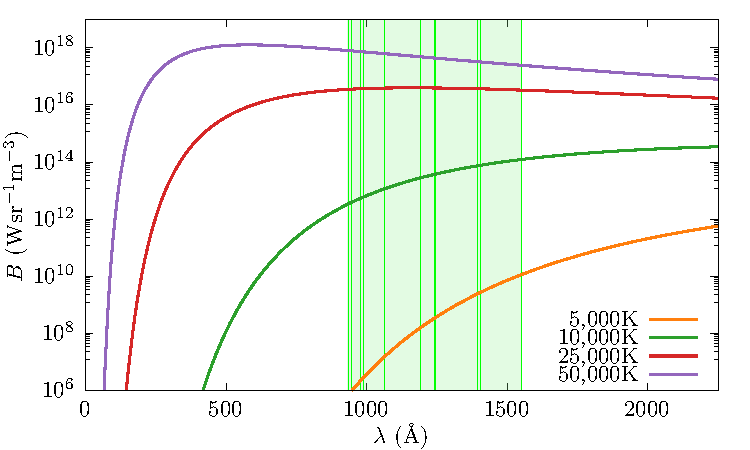
\includegraphics{assets/plancks-law/plancks-law.pdf}
  \caption[Planck's law radiance comparison with resonance lines]{Spectral radiance against wavelength for black body objects at various effective temperatures, $T_{\text{eff}}$, a series of wavelengths corresponding with important resonance lines in table 1 of \cite{lucy_mass_1970} have been included. As temperature increases the spectral radiance at resonance line wavelengths dramatically increases, with a minimum of 6 orders of magnitude difference between the effective temperatures of a solar equivalent main sequence star and an O-type main sequence or Wolf-Rayet star.}
  \label{fig:planck-comp}
\end{figure}

% Need to briefly explain P-Cygni profiles as well

% Radiative line driving, this section may need to be beefed up

Early computations involving resonance lines from \cite{lucy_mass_1970} provided a more reasonable mass loss rate calculation, but were still off by approximately two orders of magnitude.
Building off of the work by Lucy \& Solomon, a vital paper in the solidification of radiative lines as the main driving mechanism behind massive star outflows was produced by Castor, Abbott and Klein\footnote{Hereafter abbreviated as CAK.}.
The CAK formalism calculated reasonably close wind velocities, while being accurate to within a factor of 3 for mass loss rates \parencite{castor_radiation-driven_1975}.
Further work allowed for more accurate computations of the line driving effect, such as the mCAK prescription, the Sobolev approximation and the finite disk correction factor \parencite{pauldrachRadiationdrivenWindsHot1986}.

% Evolved OB stars, WR stars

As previously mentioned, evolved massive stars progress into a helium burning WR phase, at this point, mass loss rates due to radiative line driving are extreme, in the order of $10^{-5}$ \si{\solarmass\per\year}.
This outsized influence on the local medium can be seen in the production of ejecta nebula, such as M1-67 produced by WR 124 (figure \ref{fig:wr124}).

%//FIXME this is a placeholder, additionally how should I cite this?
\begin{figure}[h]
  \centering
  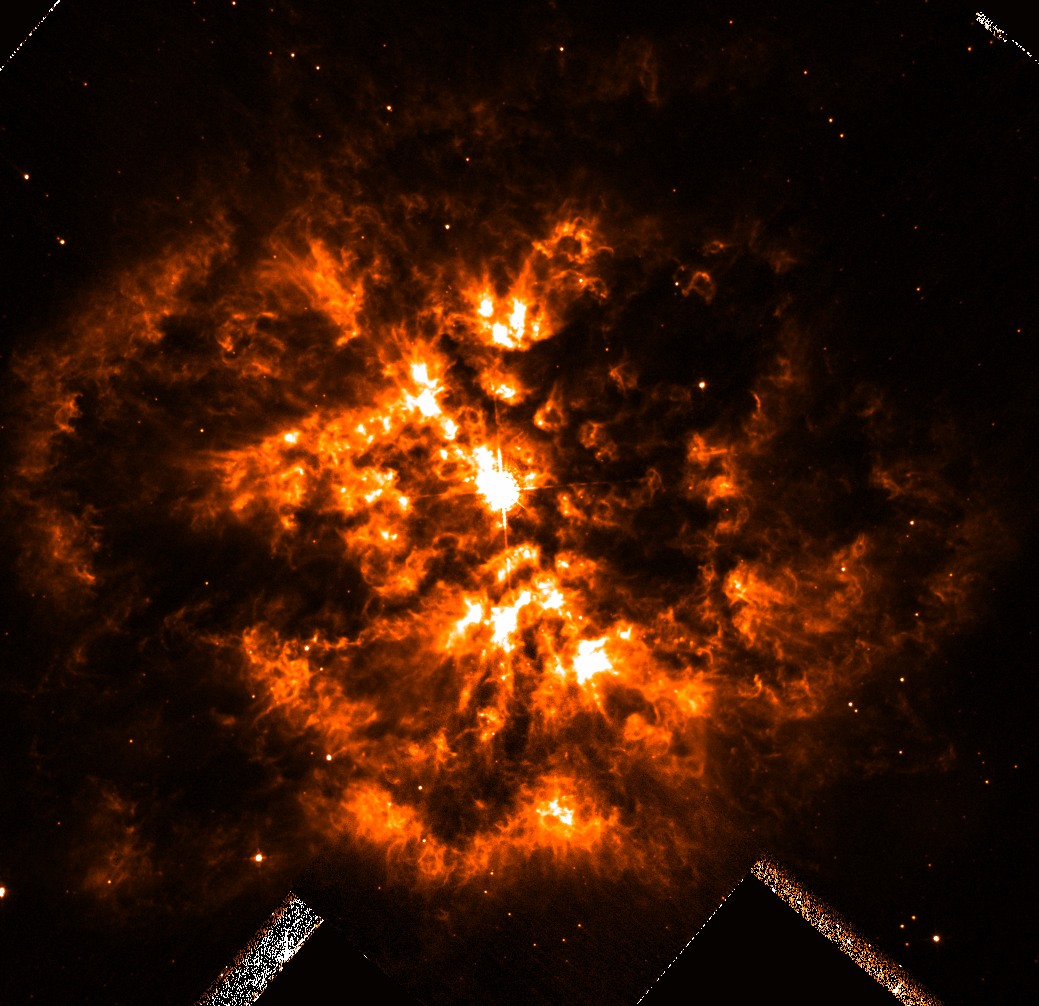
\includegraphics[width=4in]{assets/WR124.png}
  \caption[M1-67 nebula around WR 124]{Reduced Hubble WFPC2 instrument data of the WN star WR 124, its extreme mass loss is currently producing an ejecta nebula, M1-67 \parencite{2010ApJ...724L..90M}.}
  \label{fig:wr124}
\end{figure}

\begin{table}[h]
  \centering
  % \resizebox{\textwidth}{!}{%
  \begin{tabular}{cccc}
  \hline
  \multicolumn{1}{c}{Star} & \multicolumn{1}{c}{$\dot M$} & \multicolumn{1}{c}{$v_\infty$} & \multicolumn{1}{c}{Mechanism} \\
  \multicolumn{1}{c}{}     & \multicolumn{1}{c}{$\si{\solarmass\per\year}$}         & \multicolumn{1}{c}{$\si{\kilo\metre\per\second}$}           & \multicolumn{1}{c}{}          \\ \hline
  Sun            & $10^{-14}$        & 400  & Thermal heating \\
  Pre Main Sequence & $10^{-4}-10^{-7}$ & 200-500 & Rotation \& magnetic fields \\
  Red Giant      & $10^{-7}-10^{-9}$ & 30   & Radiation pressure on dust grains        \\
  OB Star        & $10^{-7}-10^{-8}$ & 2500 & Radiation pressure \& line driving      \\
  Wolf-Rayet     & $10^{-5}$         & 1500 & Radiation pressure \& line driving       \\ \hline
  \end{tabular}%
  % }
  \caption[Stellar wind comparison]{Comparison winds emitted from various types of star.}
  \label{tab:windcomp}
\end{table}

\begin{figure}
  \centering
  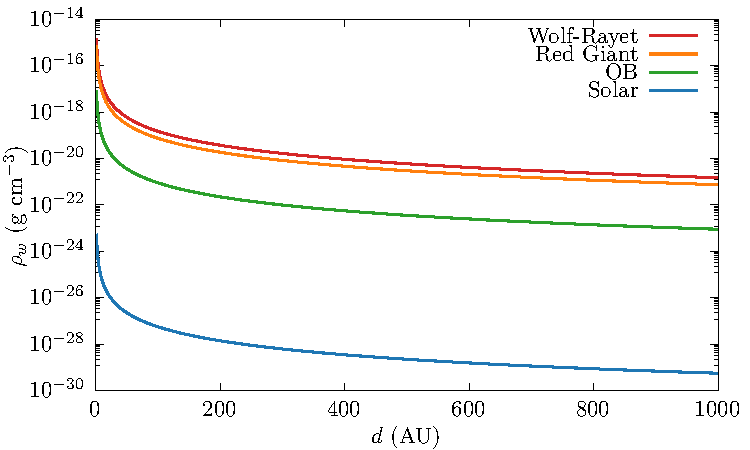
\includegraphics{assets/wind-comparison/wind-comp.pdf}
  \caption[$\rho_w$ comparison of main sequence winds]{Comparison of the densities of various main sequence winds using the parameters specified in table \ref{tab:windcomp}, wind densities are estimated using the smooth wind approximation described in equation \ref{eq:smoothwind}.}
  \label{fig:windrhocomp}
\end{figure}

\subsection{The CAK formalism}
\label{sec:cak}

\section{Interstellar Dust}
\label{sec:dust}

\subsection{The importance of interstellar dust}
\label{sec:dustimportance}

\subsection{Interstellar dust in massive star systems}
\label{sec:dustmassivestars}

\subsection{Radiation processes in interstellar dust}
\label{sec:dustcooling-background}

\section{Colliding Wind Binary Systems}
\label{sec:cwb}

% Introduction 


% //TODO Cannot get into the groove of this paragraph, please fix this future Joe
Colliding Wind Binaries\footnote{Abbreviated to CWBs.}, in opposition to all known laws of astrophysical nomenclature, is a easy to understand term - it is a binary system where stellar winds from the member stars undergoing collision.
Unfortunately, the simplicity of the systems ends here, CWB systems are extremely complex and poorly understood as they are difficult environments to observe or simulate.

%History and classification, useful sources in Stevens & Pollock 1994 

Early observations beyond visual spectrum led to the discovery of many new astrophysical phenomena, one such discovery were extremely bright persistent thermal x-ray sources, with x-ray 
The first classification and analysis of Colliding Wind Binary systems were independently performed by \cite{prilutskii_x_1976} and \cite{cherepashchukDetectabilityWolfRayetBinaries1976}, these systems were found to contain a close binary system, consisting of an evolved WR star and an OB counterpart, as their winds collide, a strong shock forms, heating the winds to temperatures in the order of $10^8$ \si{\kelvin} in the immediate post-shock environment, these extreme temperatures and the large quantity of shocked material accounted for the extremely bright thermal x-ray emission. The evidence was further compounded as the variation of the x-ray flux could be attributed to orbital motion of these binary systems.

% Analysis pollock 1987 determined binary systems\cite{pollockEinsteinViewWolfRayet1987} 

% Formation 


\subsection{The Wind Collision Region}
\label{sec:wcr}

% What is this region
The Wind Collision Region\footnote{WCR} is the most violent and turbulent region of a CWB system, a region where strong shocks lead to temperatures in excess of $10^8$ $\si{\kelvin}$.
These strong shocks contain enormous amounts of mechanical energy, in the region of $10^3$ $\si{\solarluminosity}$, WCRs are engines capable of producing huge quantities radiation through multiple thermal and non-thermal mechanisms \parencite{eichler_particle_1993,grimaldoProtonAccelerationColliding2019}.
Despite these extreme conditions, these regions are capable of producing amorphous carbon dust grains at a rate on the order \num{1e-8} \si{\solarmass\per\year}.
As these grains are extremely fragile, this is a conundrum that has plagued researchers in this field, as direct observation of the innermost regions of even nearby WCRs is difficult, bordering on impossible, much of the work in this area involves hydrodynamical simulation.

% Properties of region

%//TODO This needs a lot of work, writing equation sections is boring

% Equations
The properties of the WCR can be described by a small number of parameters.
The first of such parameters is the wind momentum ratio, $\eta$, which describes the available \parencite{usov_stellar_1991}.


\begin{equation}
  \eta = \frac{\dot M_\text{OB} v_\infty^\text{OB}}{\dot M_\text{WR} v_\infty^\text{WR}},
\end{equation}

%Theres a particular paper on improved analytical observations 

This momentum ratio can also be used to estimate the distance of the apex of the WCR to each star, using the following equations:

\begin{equation}
  r_\text{WR} = \frac{1}{1+\eta^{1/2}} , ~~~ r_\text{OB} = \frac{\eta^{1/2}}{1+\eta^{1/2}},
\end{equation}

where $r_{WR}$ is the distance from the WR star to the WCR apex, and $r_\text{OB}$ is the distance from the OB star to the WCR apex.
Work by \cite{eichler_particle_1993} goes further to utilise the momentum ratio to approximate the shape of the wind collision region, further out from the apex of the WCR, the region forms an approximately conical shape with an opening angle, $\theta_c$ of:

\begin{equation}
  \theta_c \simeq 2.1 \left(1 - \frac{\eta^{2/5}}{4}\right) \eta^{-1/3}, ~~ \text{for } 10^{-4} \leq \eta \leq 1, \label{eq:conic}
\end{equation}


% Considerations due to stagnation point flow \cite{stevens_stagnation-point_1994}

% Brief notes on astrophysical shocks, link to appendix

%Detailed breakdown of Wind collision region

\subsection{Cooling in the WCR}
\label{sec:wcrcooling}
%//TODO clean up this caption
%//TODO remove grid from plot
\begin{figure}[h]
  \centering
  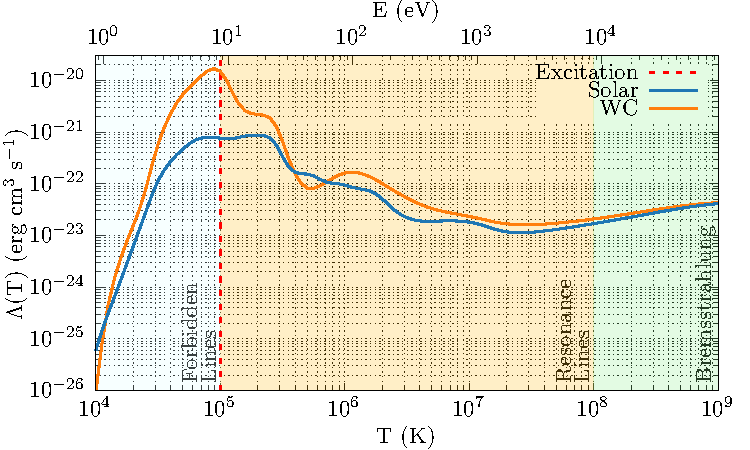
\includegraphics{assets/cooling-breakdown/cooling-curve-solar-withev.pdf}
  \caption[WC \& solar abundance plasma cooling curves]{Normalised plasma cooling rates as a function of temperature and thermal energy for solar abundance and WC abundance winds. The regions where forbidden line, resonance line and bremsstrahlung emission are dominant are highlighted, with H ionisation and recombination occuring between the forbidden and resonance line sections at $10^5$ \si{\kelvin}.}
  \label{fig:wcsolcooling}
\end{figure}

\begin{table}[h]
  \centering
  \begin{tabular}{lll}
  \\ \hline 
  \textbf{Temperature range} & \textbf{Dominant process} & \textbf{Spectral region} \\ \hline
  $\SI{5e3}{\kelvin} \lesssim T \lesssim \SI{1e5}{\kelvin} $ & Forbidden lines & IR, Optical \\
  $T \approx \SI{1e5}{\kelvin}$ & H excitation/ionisation & Optical, UV \\
  $\SI{5e3}{\kelvin} \lesssim T \lesssim \SI{1e5}{\kelvin} $ & Resonance lines & Far UV, soft X-ray \\
  $T \gtrsim \SI{1e8}{\kelvin} $ & Bremsstrahlung & Radio \\ \hline
  \end{tabular}
  \caption[Cooling processes at various temperature ranges]{Breakdown of dominant cooling processes at various temperature ranges from \cite{dysonPhysicsInterstellarMedium2021}, whilst H excitation/ionisation occurs over a very short temperature range, it is extremely influential, causing a global peak in the cooling rate at $\approx 10^5$ \si{\kelvin}. These temperature ranges are depicted in figure \ref{fig:wcsolcooling}.}
  \label{tab:coolprocess}
  \end{table}

% Radiative cooling, include graphs, mechanisms

Cooling due to radiation emission in a hot plasma can be broken down into a variety of processes that occur over series of temperature ranges.
Ions inside a plasma can become excited through collisions or photon absorption resulting in emission of photons as the ions de-excited. 

Mechanisms that are significant within the warm\footnote{See what I mean about the phrase ``warm''?} and hot gas phases include forbidden line emission, hydrogen excitation and ionisation, resonance lines and bremsstrahlung, the influence of each mechanism waxes and wanes as temperature increases, with each mechanism clearly dominant over \parencite{dysonPhysicsInterstellarMedium2021}.

% Section on forbidden line emission

The first mechanism to be discussed is forbidden line emission\footnote{Like many other phenomena discussed in this thesis, this too is a misnomer, while initially assumed to be prohibited under the contemporary understanding of atomic physics, it is in fact just astrophysicists jumping the gun again.}.
This process dominates the cooling process of cooler gas that is not fully ionised, where collisions with free electrons excite metals within the gas, causing them to de-excite through photon emission through these forbidden lines.
Forbidden lines themselves arise from magnetic dipole and quadrupole fine structure states within typical energy levels, despite having a much lower probability of occurring compared to conventional energy level transitions.
This process dominates at these temperatures as the transition energies are significantly lower, on the order of 1 \si{\electronvolt}, as the photon is also of a comparatively long wavelength, it can more easily escape from the gas without being re-absorbed by it.

% Section on ionisation/recombination

As the temperature increases there is a spike in the cooling rate of the gas as the hydrogen present begins to fully ionise, at this temperature a hydrogen ion and an electron may recombine, releasing a cascade of photons as the electron de-excites.

% Section on resonance line emission

As the plasma heats further resonance lines can

% Section on braking radiation

As the particle energy reaches the range of tens of \si{\kilo\electronvolt}, bremsstrahlung\footnote{Or braking radiation when you can't remember how to spell it.} becomes dominant (figure \ref{fig:wcsolcooling}). High velocity electrons are deflected by ions, emitting radiation in the process due to conservation of energy. 

% \parencite{1993ApJS...88..253S}
\parencite{schureNewRadiativeCooling2009}
\parencite{rybickiRadiativeProcessesAstrophysics2004}




%//TODO clean up this caption
%//FIXME use the new cooling code for this graph, early changes in ionisation fraction result in a different appearance from 1e4 to 1e6 kelvin!
\begin{figure}
  \centering
  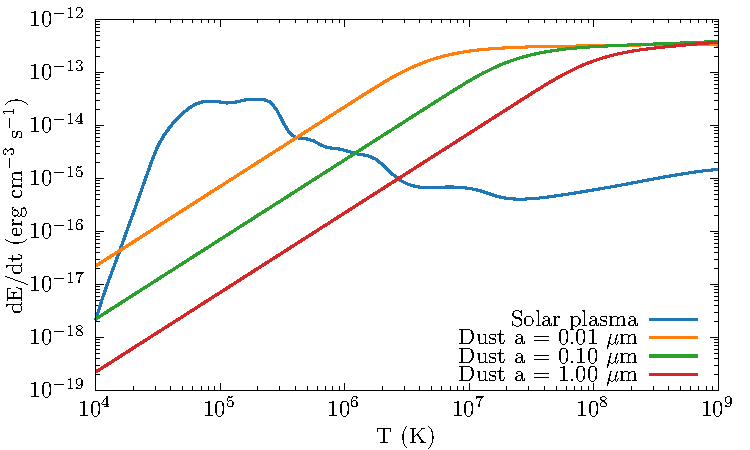
\includegraphics{assets/dust-plasma-cooling-comparison/cooling-comparison.pdf}
  \caption[Dust cooling vs. plasma cooling]{Comparison of plasma cooling to dust cooling with different grain sizes in a solar abundance gas, where $\rho_g = 10^{-20}$ \si{\gram\per\centi\metre\cubed} and a dust-to-gas mass ratio of 0.01.}
  \label{fig:dustplasmacomparison}
\end{figure}

% Needs to be spun off into a subsection

% Cooling parameter

\begin{subequations}
  \begin{align}
    \tau_\text{cool} & = \frac{k_B T_s}{4n_w \Lambda(T_s)} \label{eq:taucool} ,\\ 
    \tau_\text{esc}  & = \frac{d_\text{sep}}{c_s} \label{eq:tauesc} ,
  \end{align}
\end{subequations}

\begin{equation}
  \chi = \frac{\tau_\text{cool}}{\tau_\text{esc}} \approx \frac{v^4_{\infty,8} d_\text{sep,12}}{\dot M_{-7}} \label{eq:coolingparameter} ,
\end{equation}

% Dust cooling? Might need to move CWB dust formation up
The presence of dust within the immediate post-shock environment significantly increases the cooling rate.
Figure \ref{fig:dustplasmacomparison} compares rate of cooling due to dust emission of various types of grains to plasma cooling at solar abundances, 
As $\Lambda_g$ and $\Lambda_D$ are both proportional to $\rho_g^2$, dust cooling will dominate at high temperatures so long as there is sufficient amounts of dust.
%//TODO Lengthen paragraph, introduction to dust cooling

As dust grains collide with ionised gas and electrons, this imparts kinetic energy into the grains, heating them and causing them to emit infrared radiation. Assuming that there is a net accretion of ions and electrons onto the dust grains and the gas is optically thin in the infrared regime, energy is efficiently removed from the gas.
At particularly high temperatures this effect can dominate over high-temperature plasma cooling processes such as bremsstrahlung, as seen in figure \ref{fig:dustplasmacomparison}.
Figure \ref{fig:collisionalheatingcomparison} compares dust grain heating rates due to electron and ion collisional excitation in a solar abundance and WC abundance flow.
At lower temperatures the dust grain cooling rate is dominated by electron excitation, especially in the WC case as the ratio of free electrons to ions is significantly higher, as the WC flow is enriched by heavier elements.
However, as the grain temperature increases, collisional heating due to ions becomes more prevalent as the electrons are sufficiently energetic to pass through the grain without significant energy transfer; this is referred to as the electron transparency, $h_e$ \parencite{dwek_infrared_1981}.

\begin{figure}[h]
  \centering
  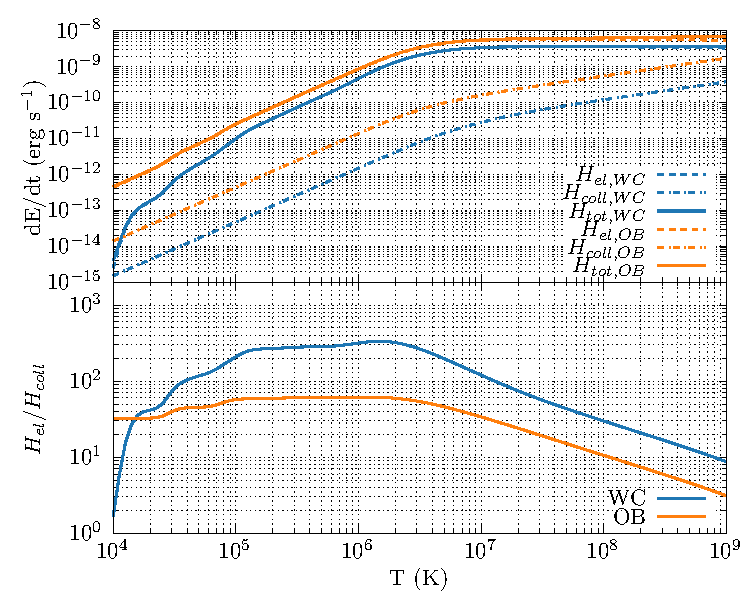
\includegraphics{assets/dust-electron-contribution/coll-el-comp.pdf}
  \caption[$H_{el}$ and $H_{coll}$ comparison]{Comparison of grain heating rate due to ion collisional excitation, $H_{coll}$, and electron excitation, $H_{el}$. The dust grain has a grain radius of \SI{5e-3}{\micro\metre} and is travelling through a gas with a density of $10^{-20}$ \si{\gram\per\centi\metre\cubed} with solar and WC abundances.}
  \label{fig:collisionalheatingcomparison}
\end{figure}


Work by \cite{dwek_infrared_1981} is used predominantly in this project to simulate cooling due to dust, a fast method for calculating the cooling rate due to dust was integrated into the numerical code for this project, which is elaborated on in section \ref{sec:dustcoolingmodel}.
% Finish and link to below paragraph

%Find citation for spitzer 1978

The heating rate of a dust grain due to collisions 

\begin{equation}
  \begin{split} 
      H_\text{coll} = & n \pi a^2 \langle Q(E,q,U) \rangle \\
      & \times \langle v (E-qU) f(a,E-qU) f(a,E-qU) \rangle \, \si{\erg\per\second}
  \end{split}
\end{equation}

%Explain constants
This can be simplified and expressed in the equation:

\begin{equation}
  \begin{split}
    H_\text{coll} & = \left(\frac{32}{\pi m}\right)^{1/2} n\pi a^2 (k_B T)^{3/2} h(a,T) \\
    & = \num{1.26e-19} \frac{n}{A^{1/2}} a^2 (\si{\micro\metre}) T^{3/2} h(a,T) \, \si{\erg\per\second}
  \end{split}
\end{equation}

% This part is very dry and is going to explain the equations more in depth
% Main source will be dwek 1981 appendix 2



% Instabilities due to cooling, might spin off into it's own appendix chapter?
% Theres a particular paper that covers this 
% Mainly need to discuss KH instabilities, and how they relate to cooling



\subsection{Dust formation in CWB systems}
\label{sec:cwbdust}

%Intro to dust formation in said systems

%Observational data Link to Williams papers in particular, dust formations only around WC

%Theories as to why


\subsection{Important WCd systems}

% This might be a good section?
\subsection{Contemporary research in extragalactic low-metallicity WCd systems}

\label{sec:knowndustysystems}

